In Section~\ref{sec:similarity-study}, we presented a brief study
of content similarity in the IODEDUP traces available online 
at \cite{iodedup-online}, by presenting 
metrics like the ``sharing'' factor and the content ``occurrence'' factor
in the traces. In this section, we perform a more detailed study
to capture more characteristics of the workload
which can be used for synthetic generation of realistic
benchmarks, in future.

We characterize the \textit{webvm} and \textit{homes} traces from \cite{iodedup-online}
using the following four major
metrics for both read and write requests separately. Note that, I/O
deduplication techniques attempt to optimize only the disk read performance,
so it would be preferable to capture the disk read and write characteristics
of the trace separately, rather than together. 
\begin{enumerate}
		\singlespacing
	\item Blocks accessed distribution
	\item Run length distribution
	\item Reuse distribution
	\item Jump length distribution
\end{enumerate}

For each of the above metrics, we first present a basic definition 
accompanied by an example and then present the characterization of the
traces based on that metric. Along-with the block-based interpretation of
the metric, we also present the ``content-based interpretation'', the point
being that I/O deduplication is to be performed for traces that have
duplicate content so the content-defined trace characterization is especially
relevant.

 \begin{table}[t]
 \caption{Summary statistics of one week I/O workload traces \textit{webvm} and \textit{homes}~\cite{iodedup}}
%  \hspace{-0.2in}
 \begin{center}
 \begin{tabular}{|c|c|c|c|c|} \hline
   \bf{Workload} & \bf{Filesystem} & \bf{Memory} & \bf{Filesystem} & \bf{Filesystem size} \\
  \bf{type} & \bf{size (GB)} & \bf{size (GB)} & \bf{accessed (\%)} & \bf{(no. of 4KB blocks)} \\ \hline
  \textit{webvm} & 70 & 2 & 2.8 & 18 million \\
  \textit{homes} & 470 & 8 & 1.44 & 123 million \\ \hline
 \end{tabular}
 \label{tab:tracechar-summary-stats}
 \end{center}
 \end{table}
 

Before presenting the distributions, we present summary
statistics regarding the traces considered in 
Table~\ref{tab:tracechar-summary-stats}\textemdash{}these are statistics reproduced
from the original paper~\cite{iodedup}.
As can be seen in the table, \textit{webvm} trace is from a filesystem of size only 70 GB
whereas \textit{homes} trace has a filesystem of size 470 GB backing it. This implies
that the range of block addresses accessed in the latter filesystem is expected
to be greater than the former. The primary memory allocated in both systems
is also different\textemdash{}2 GB and 8 GB, respectively. Thus, the \textit{homes} trace
has been captured downstream of a much bigger cache than the \textit{webvm}
trace\textemdash{}this may be partly the reason why the \textit{homes} trace does not
seem to have much duplicate content to be exploited by the I/O deduplication
techniques (refer Fig.~\ref{fig:similarity-distrib} in Section~\ref{sec:similarity-study}).

In Table~\ref{tab:tracechar-summary-stats}, the percentage (\%) of 
filesystem accessed indicates that in both concerned systems, 
the total number of block addresses accessed in the trace constitutes only
a small fraction of the entire file system size. This implies that if the
metadata is constructed dynamically (i.e., while the application is 
executing), it needs to represent only that portion
of the filesystem that is accessed in the workload, and not the whole filesystem.
Note that, this requirement is different from that of a storage deduplication
system which needs to persistently retain metadata regarding the entire data
within the system.


 
For trace characterization, we consider the entire three-week \textit{webvm}
and \textit{homes} trace, and report various distributions (instead
of averages) in accordance with the insight in 
\cite{commercial-characterization} that ``distribution matters, not 
the average''. 

\subsection{Blocks accessed distribution}

%These figures were plotted directly from Octave, and hence having all
%this problem. The only thing good in Octave was that it could easily
%plot histogram with 25 bucket by hist(X, 25). Plotting has been a real
%pain though, so better to use [y, x] = hist(X,25) and then print out
%the x and y values, to use them separately in a gnuplot script with
%desired formatting.
%\hspace{-1in}
\begin{figure}[t]
	\centering
	\subfloat[Access distribution of blocks read (\textit{webvm})]{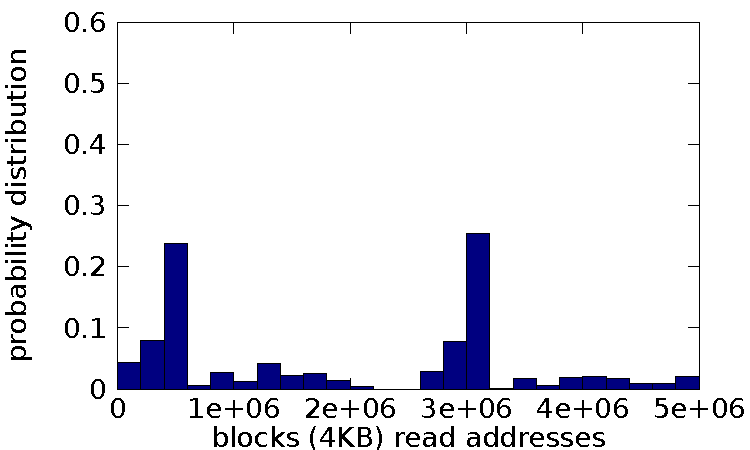
\includegraphics[scale=0.6]{tracechar-figures/21-day/webvm-block-read-appended-21-prob.pdf}}
	\hfill
	\subfloat[Access distribution of blocks written (\textit{webvm})]{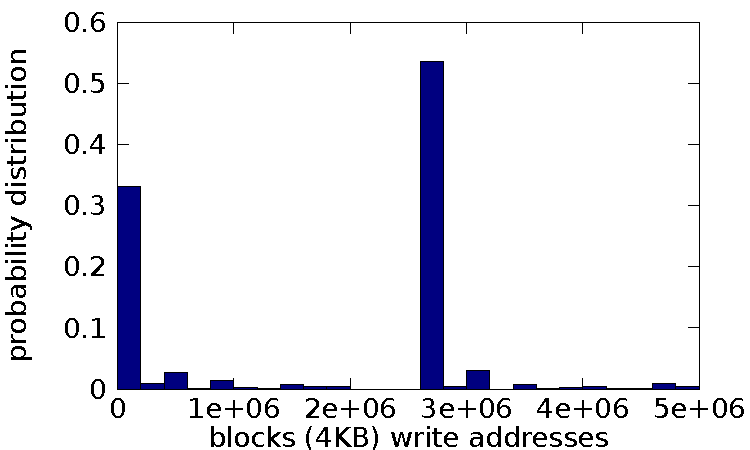
\includegraphics[scale=0.6]{tracechar-figures/21-day/webvm-block-write-appended-21-prob.pdf}}
	\\
	\subfloat[Access distribution of blocks read (\textit{homes})]{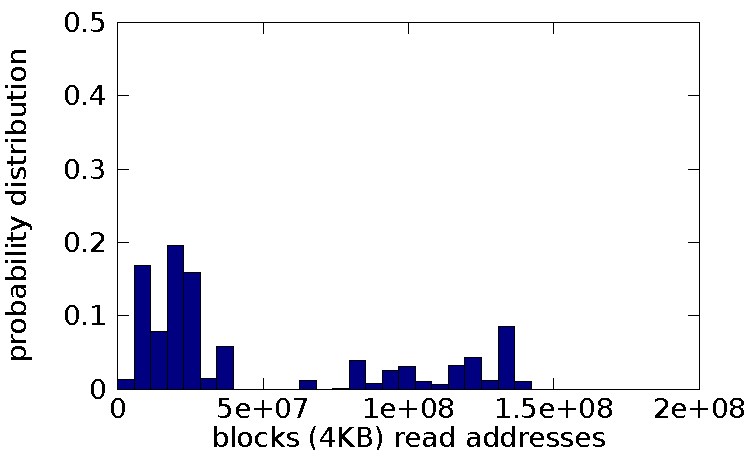
\includegraphics[scale=0.6]{tracechar-figures/21-day/homes-block-read-appended-21-prob.pdf}}
	\hfill
	\subfloat[Access distribution of blocks written (\textit{homes})]{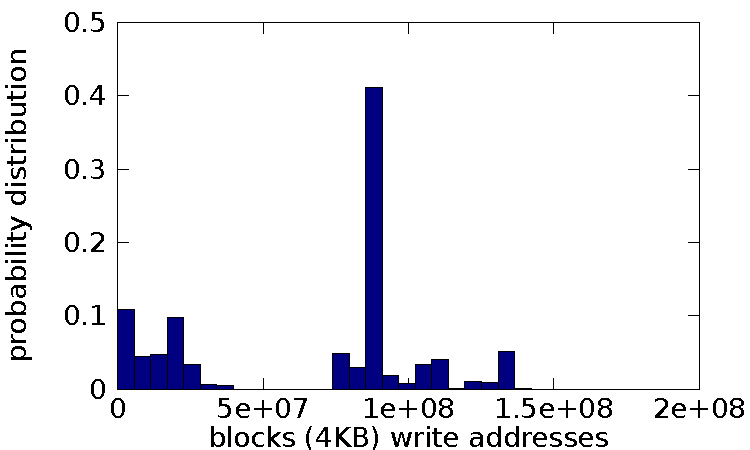
\includegraphics[scale=0.6]{tracechar-figures/21-day/homes-block-write-appended-21-prob.pdf}}
	\caption{Block access popularity distribution for reads and writes in 
	\textit{webvm} and \textit{homes} traces}
	\label{fig:webvm-blocks-read-write-distrib}
\end{figure}

%\hspace{-0.7in}
%\begin{minipage}[t]{0.6\textwidth}
%\begin{figure}
%	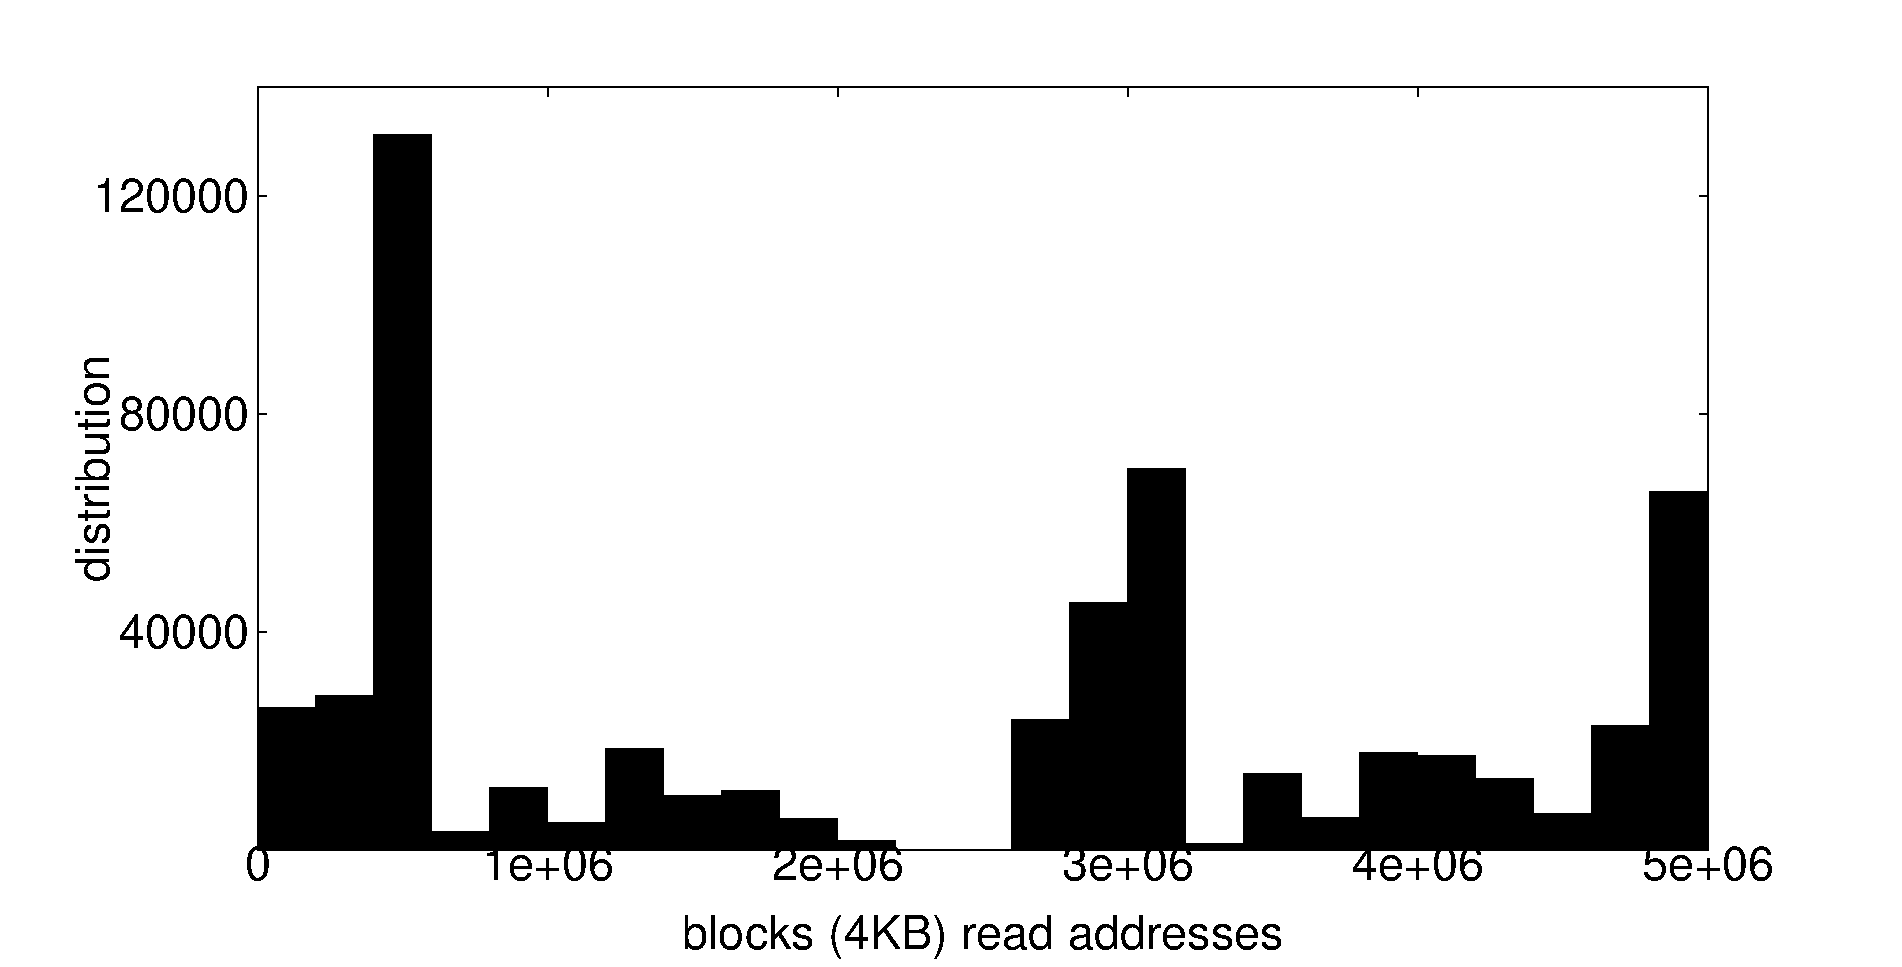
\includegraphics[width=\textwidth]{tracechar-figures/3-day/webvm-block-read-appended-3.eps}
%	\label{fig:webvm-block-read-distrib}
%	\caption{Distribution of blocks read}
%\end{figure}
%\end{minipage} 
%\hfill
%\begin{minipage}[t]{0.6\textwidth}
%\begin{figure}
%	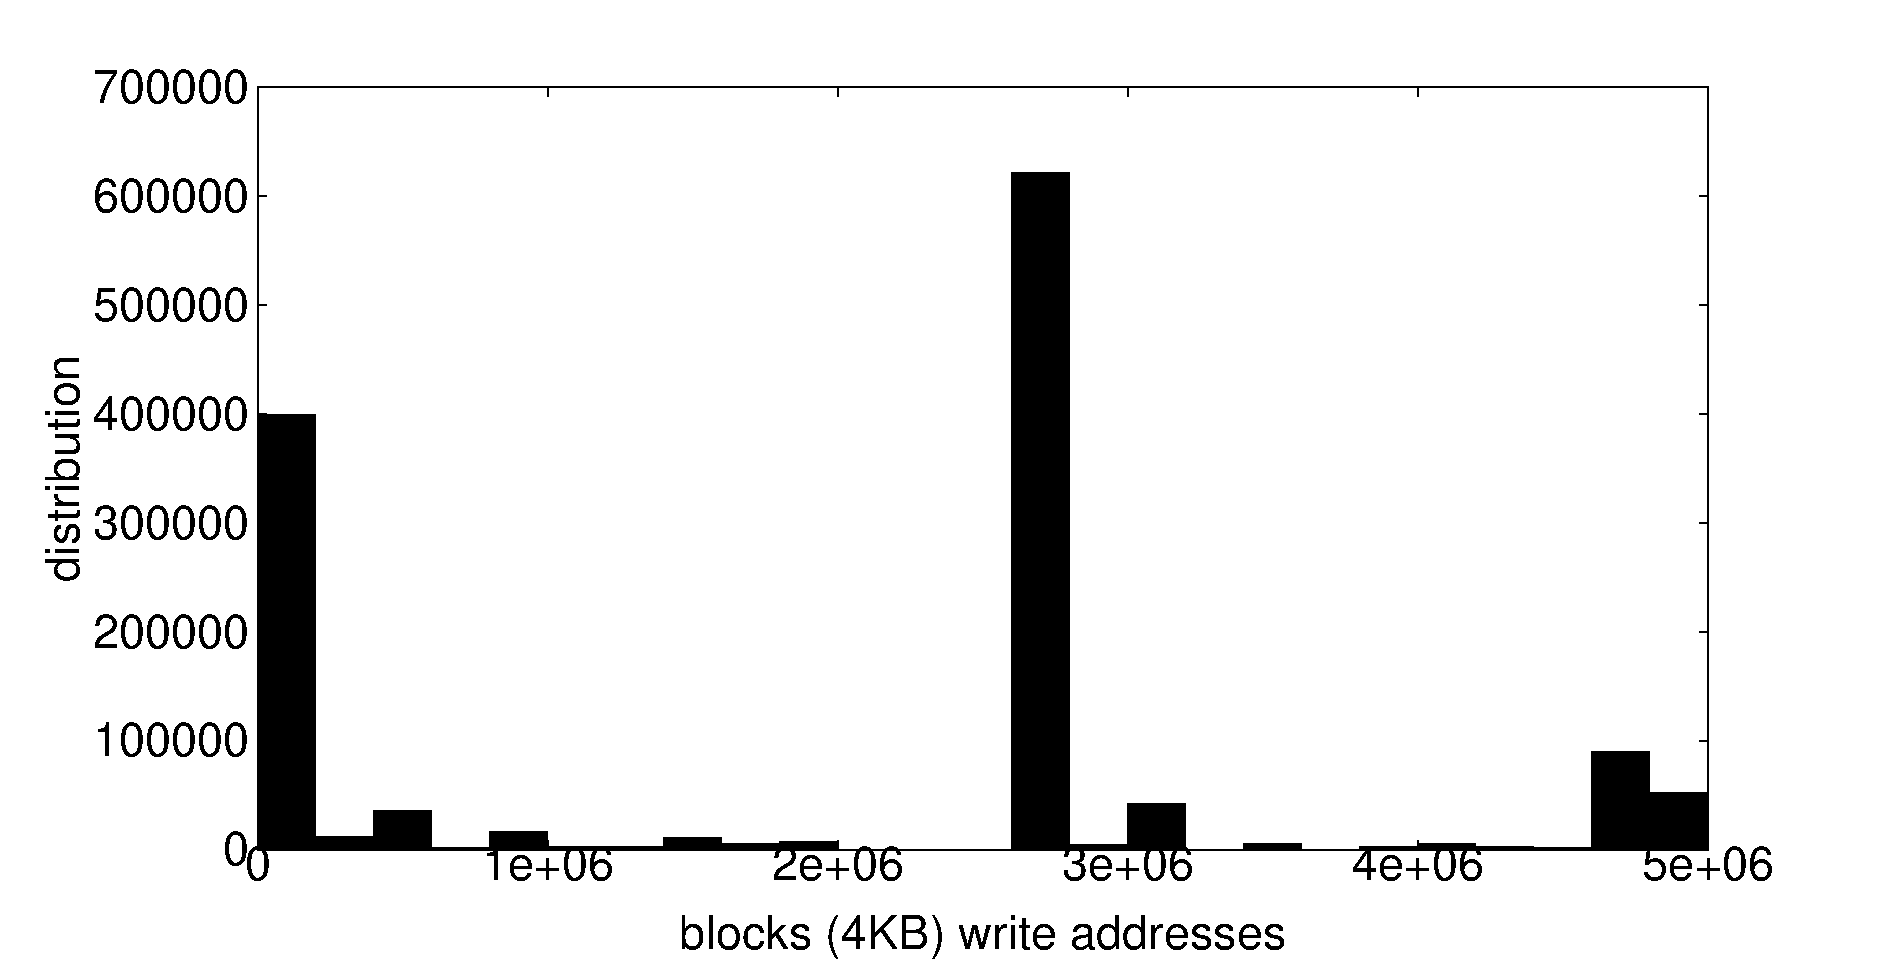
\includegraphics[width=\textwidth]{tracechar-figures/3-day/webvm-block-write-appended-3.eps}
%	\label{fig:webvm-block-write-distrib}
%	\caption{Distribution of blocks written}
%\end{figure}
%\end{minipage}

%\begin{figure*}
%	\centering
%	\vspace{-1.2in}
%	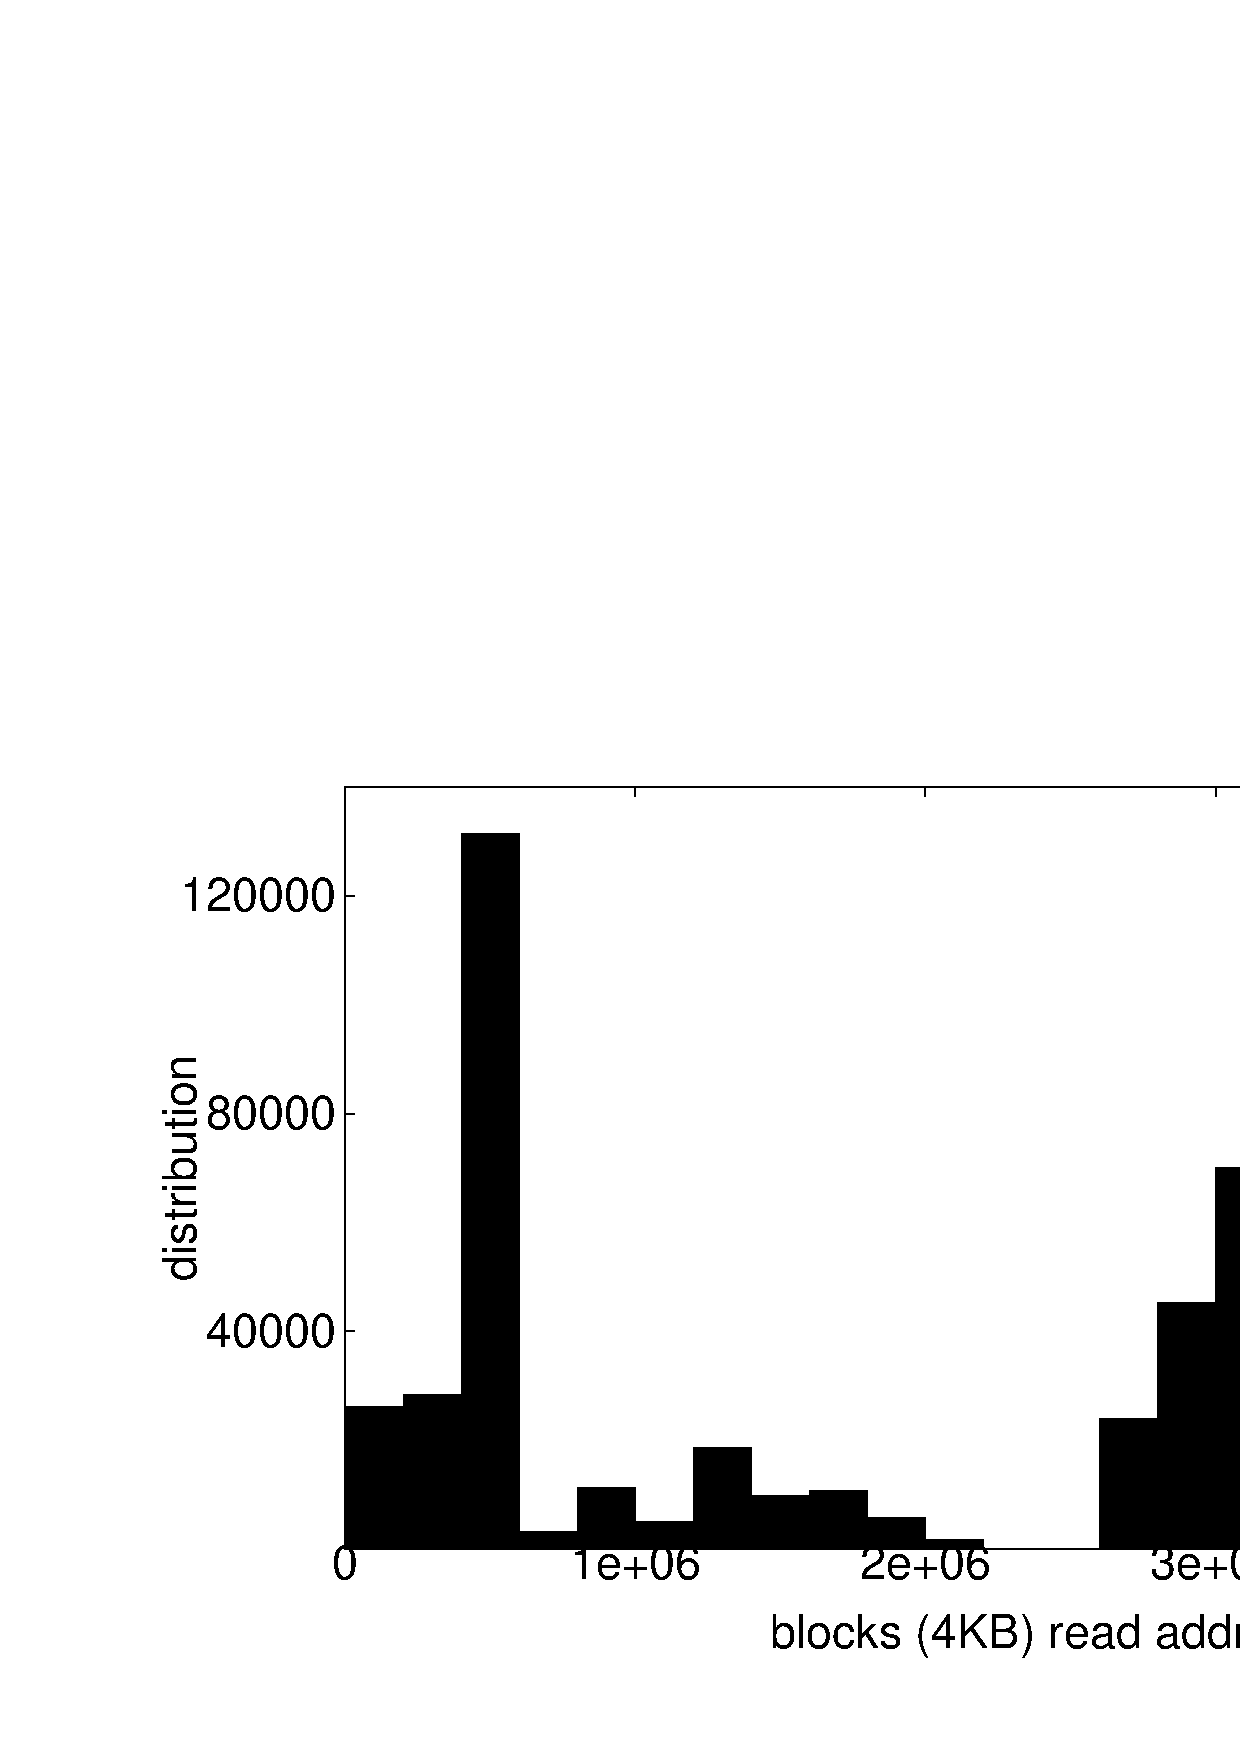
\includegraphics[scale=0.40]{tracechar-figures/3-day/webvm-block-read-appended-3.pdf}
%	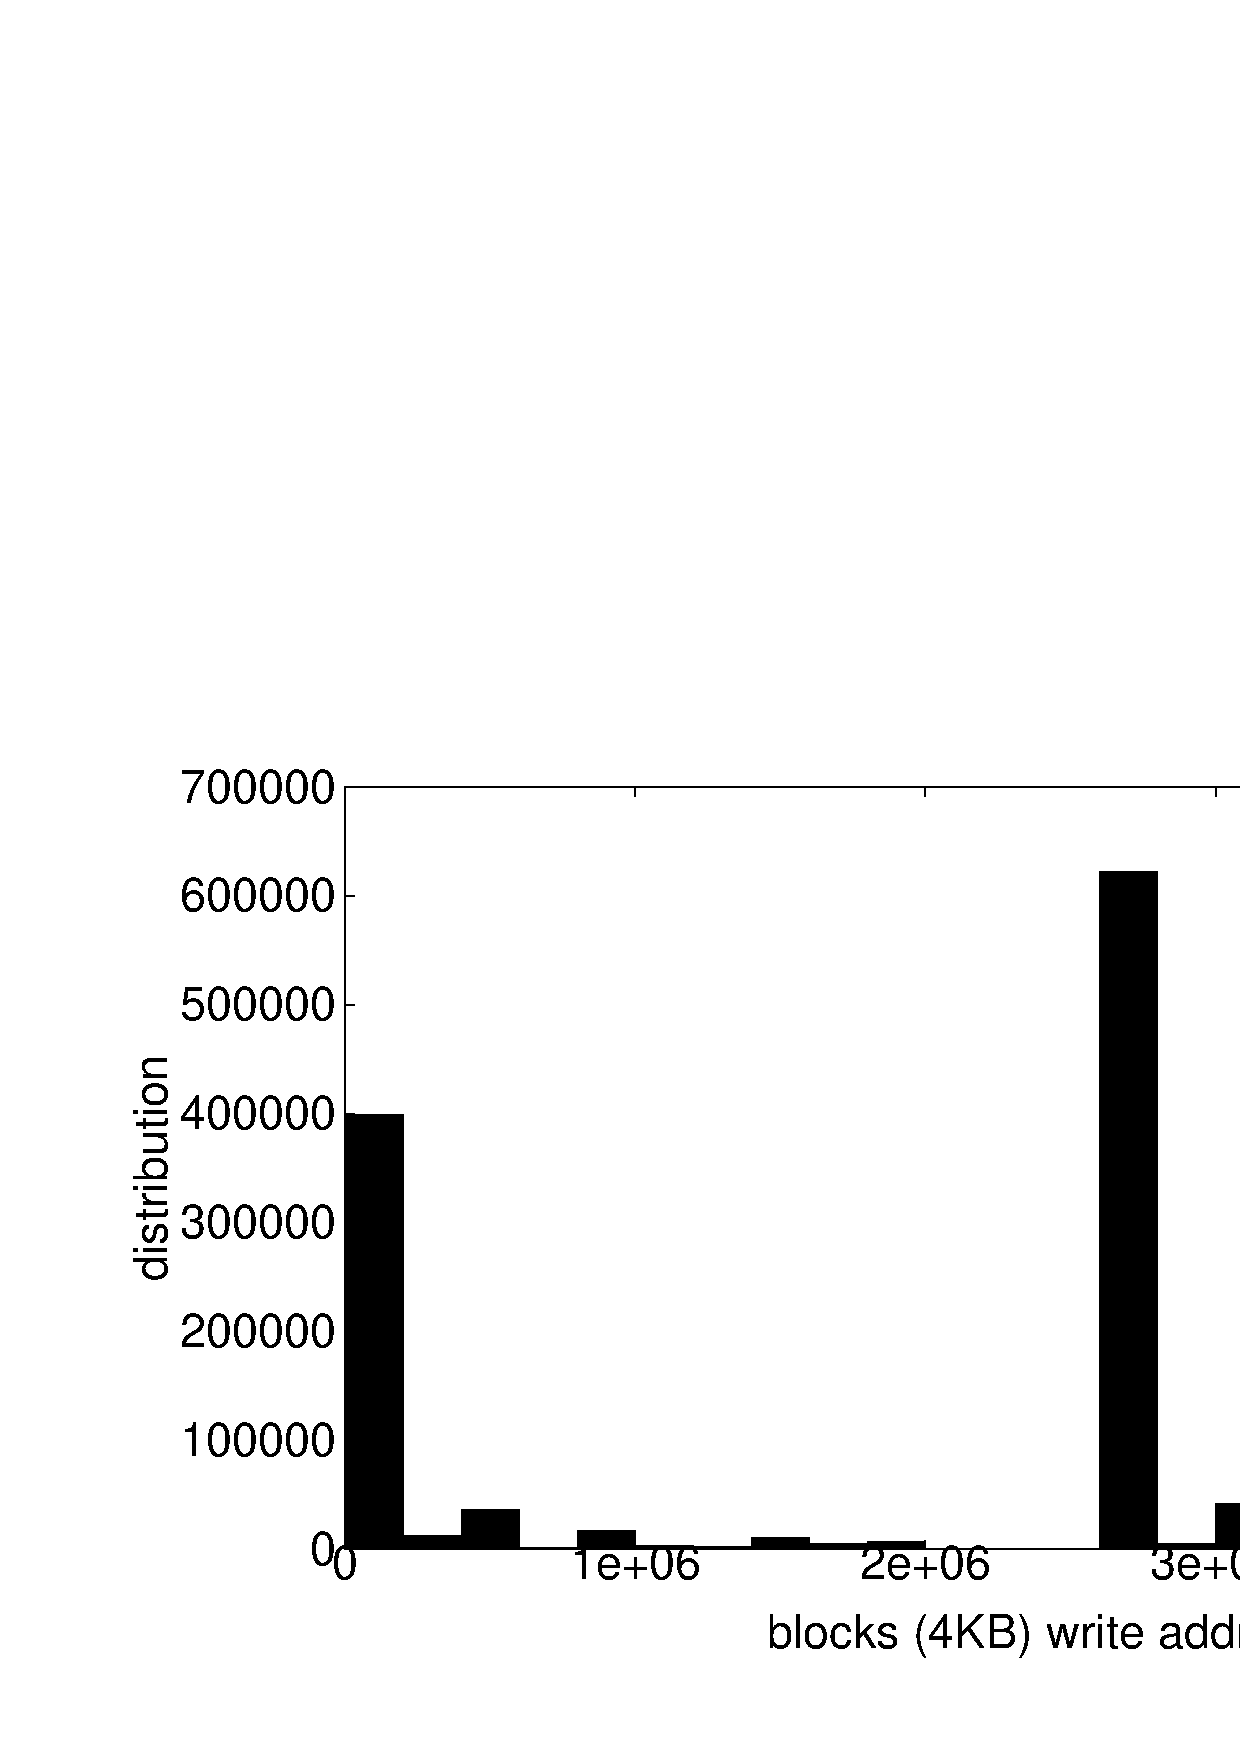
\includegraphics[scale=0.40]{tracechar-figures/3-day/webvm-block-write-appended-3.pdf}
%	\vspace{-1.2in}
%	\caption{Distribution of blocks read and written for the \textit{webvm} trace}
%	\label{fig:webvm-blocks-read-distrib}
%\end{figure*}

Fig.~\ref{fig:webvm-blocks-read-write-distrib}(a) presents a probability distribution 
of the 4KB block addresses read in the \textit{webvm} trace, 
while Fig.~\ref{fig:webvm-blocks-read-write-distrib}(c) presents the same
for the \textit{homes} trace. The x-axis plots the addresses of the blocks 
read or written, respectively, such that each address is for a 4 KB block 
or 8 sectors or 4096 bytes. 
It can be seen that a major portion of
the read accesses in both traces are limited to only some portions of the address space, 
while the rest of the address space gets much fewer read accesses. 
Similar behaviour is observed in the write accesses as well, as shown
in Fig.~\ref{fig:webvm-blocks-read-write-distrib}(b)
and Fig.~\ref{fig:webvm-blocks-read-write-distrib}(d), respectively. 
% Note that, though the
% x-axis limits are the same for both the read and write graphs, the y-axis ranges 
% are different\textemdash{}this is in line with the fact that the total number
% of reads in both the traces is lower than the number of writes.
Note that, the total range of blocks accessed is bigger in case of
the \textit{homes} trace as compared to the \textit{webvm} trace\textemdash{}this is
because the file system size in case of the former is around an order
larger than the latter, as shown in 
Table~\ref{tab:tracechar-summary-stats}.

The above block accessed distributions prove that there is \textit{spatial locality} in
the blocks being accessed in the traces, i.e., the accesses tend to be clustered more
in particular regions instead of being uniformly distributed throughout the address
range. This behaviour is typical of most storage I/O workloads and several
models have been proposed in literature to capture this characteristic
into realistic benchmarks~\cite{jump-based-synthetic, storagecharacterization, storagemodeling,
storagereplay}.

Fig.~\ref{fig:webvm-blocks-read-write-distrib} refers to all (i.e., unique as well as
duplicate) blocks
being accessed in the trace, however since we are interested in I/O
deduplication, it would be interesting to know whether such spatial 
locality of access exists for duplicate data as well. The work in
\cite{idedup} certainly demonstrates this to be true of real-world storage content,
however the question that faces us is whether this is true of I/O workloads 
as well.
\begin{figure}
	\centering
	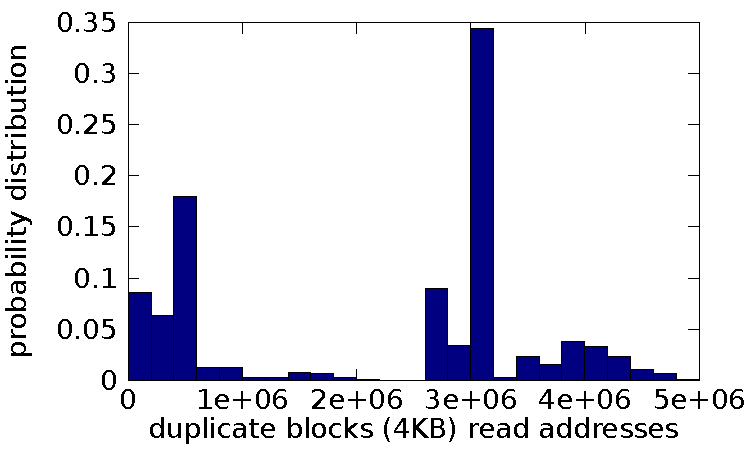
\includegraphics[scale=0.6]{tracechar-figures/21-day/webvm-dedup-block-read-appended-21-prob.pdf}
	\caption{Distribution of accesses of duplicate content blocks}
	\label{fig:webvm-blocks-dedup-distrib}
\end{figure}


To answer the question of spatial locality in duplicate content, we 
consider only those records from the trace which read ``duplicate''
data, i.e., each trace record considered in this scenario is associated
with content that has already been read or written in a previous trace
record. For every block of content that we encounter in the trace, we
assign it an index called the \texttt{dedupID} and if a content is
repeated, it is assigned the same \texttt{dedupID} as the previous
instance of that content in the trace. Thus, \texttt{dedupID} is a
unique identifier for block content, and in 
Fig.~\ref{fig:webvm-blocks-dedup-distrib}
we plot the access distribution for only those content which were 
found to be duplicate in the \textit{webvm} trace.
As expected, we can see in Fig.~\ref{fig:webvm-blocks-dedup-distrib}
that there is spatial locality within the accesses
of duplicate data as well. 
Thus, our observations echo those present in \cite{idedup}.

% Below reasoning based on WRONG input... had accidentally thought that rw=1! meant write...
% However, note that the number of duplicate 
% content instances seems to be much smaller compared to the total number
% of blocks read. Given this observation, one would wonder
% how DRIVE system is able to achieve the significant performance improvement 
% that we observed in Section~\ref{sec:drivechap-experimental-eval}. The
% reason is that DRIVE evaluation was performed over the entire three 
% week long trace, whereas these distributions have been presented only for
% the trace of the first 3 days therein. This trace snippet has 
% around 550K (556539) reads and 1300K (1328233) writes, giving a total
% of around 1850K (1884772) block trace records.

% As can be seen in 
% Fig~\ref{fig:contentdedup-factor-timeseries} of 
% Section~\ref{sec:drivechap-experimental-eval},
% the content deduplication in DRIVE system really starts performing
% significantly well
% only much later during the trace replay. This indicates that the 
% \textit{webvm} trace most likely has higher levels of duplicate content
% access in the later days' traces than the earlier days. This further
% hints that using small synthetic benchmarks is unlikely to prove DRIVE's
% performance benefits, as opposed to evaluation on realistic 
% long-running benchmarks.

\subsection{Run length distribution}
In general, run length refers to the length of a sequential run. In the
context of I/O traces, \textit{run length} refers to the length of 
a sequence of blocks being requested. For example, if the block accesses
occur as shown in Fig.~\ref{fig:runlength-example}, the first sequence
of block accesses results in a run length of 2, the second sequence has
a run length of 5, and the third sequence has a run length of 1. 

\begin{figure}
	\centering
	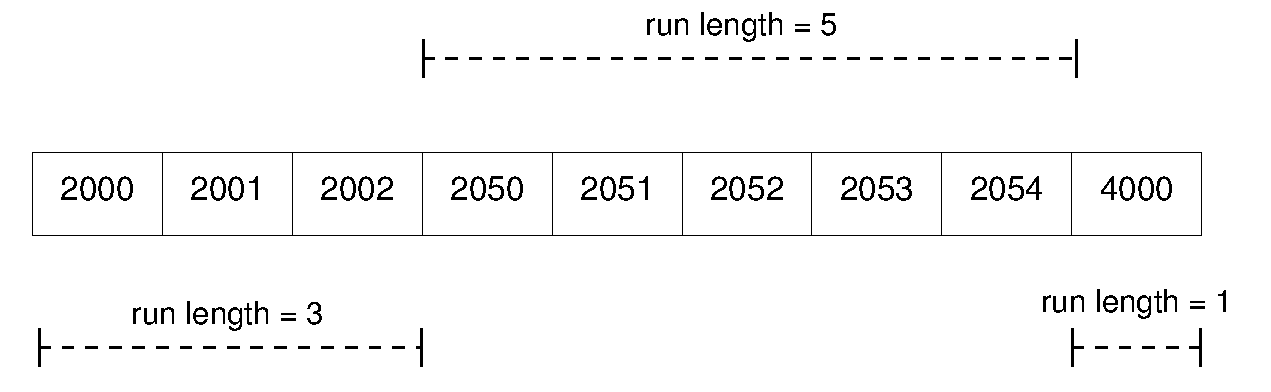
\includegraphics[scale=0.55]{tracechar-figures/21-day/runlength-example.pdf}
	\caption{Example to explain the definition of \textit{run length}}
	\label{fig:runlength-example}
\end{figure}

For \textit{webvm} trace characterization, we present its run length
distribution, i.e., a distribution of the different length sequences
in the trace. This metric will indicate whether the requests in the
trace have the sequentiality property, or whether they are essentially
random access. It may be noted that if there are many huge files being
accessed or read from the file system, it will cause bigger run lengths
to be recorded in the trace. On the other hand, if the files being read are 
small (i.e. less than 4KB in size), then the read workload will seem to be
random instead of sequential, since entire files
each will get read in a single I/O~\cite{animation-nfs}.

\begin{figure}[t]
	\centering
	\subfloat[Block run length for reads (\textit{webvm})]{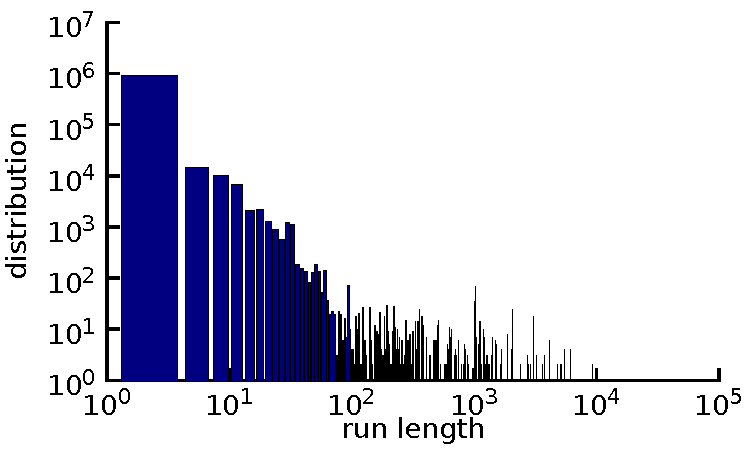
\includegraphics[scale=0.6]{tracechar-figures/21-day/webvm-run-length-distrib-readonly-appended-21-loglog.pdf}} 
	\hfill
	\subfloat[Block run length for writes (\textit{webvm})]{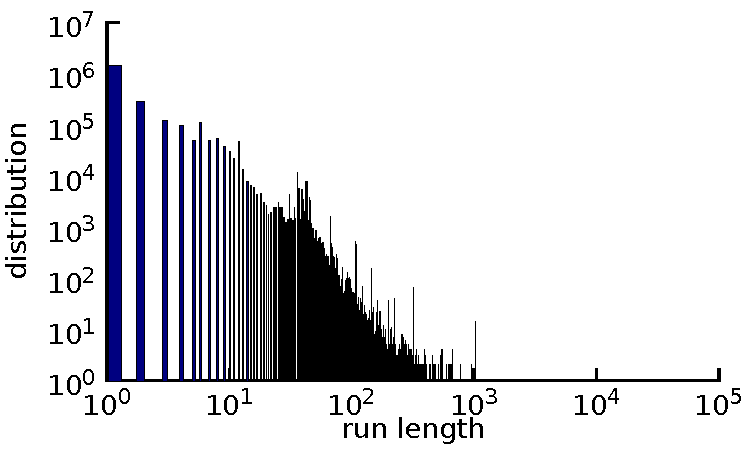
\includegraphics[scale=0.6]{tracechar-figures/21-day/webvm-run-length-distrib-writeonly-appended-21-loglog.pdf}}
	\\
	\subfloat[Block run length for reads (\textit{homes})]{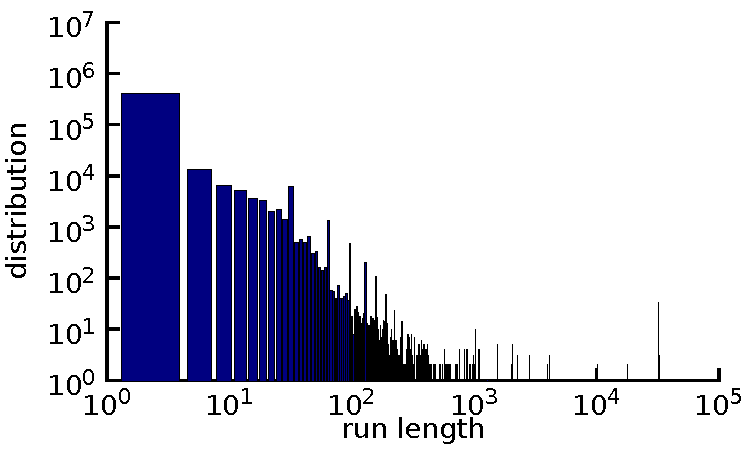
\includegraphics[scale=0.6]{tracechar-figures/21-day/homes-run-length-distrib-readonly-appended-21-loglog.pdf}} 
	\hfill
	\subfloat[Block run length for writes (\textit{homes})]{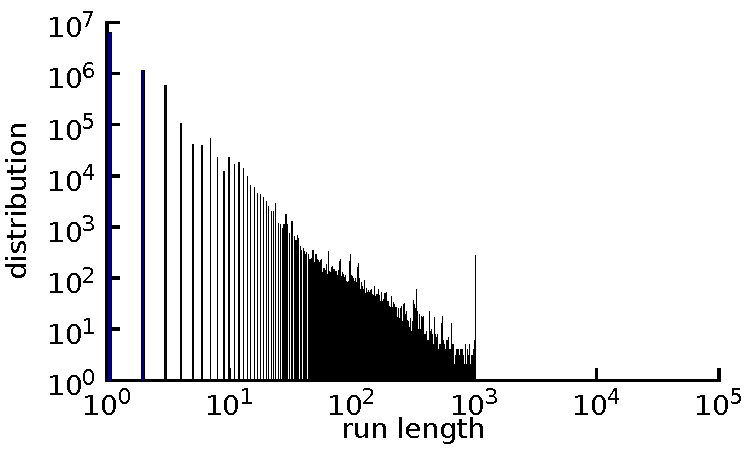
\includegraphics[scale=0.6]{tracechar-figures/21-day/homes-run-length-distrib-writeonly-appended-21-loglog.pdf}}
	\caption{\textit{Block run length} distribution for reads and writes in \textit{webvm} and \textit{homes} traces}
	\label{fig:webvm-runlength-read-write-distrib}
\end{figure}



%\begin{figure}[t]
%	\centering
%	\subfloat[Run length for duplicate content blocks accessed consecutively]{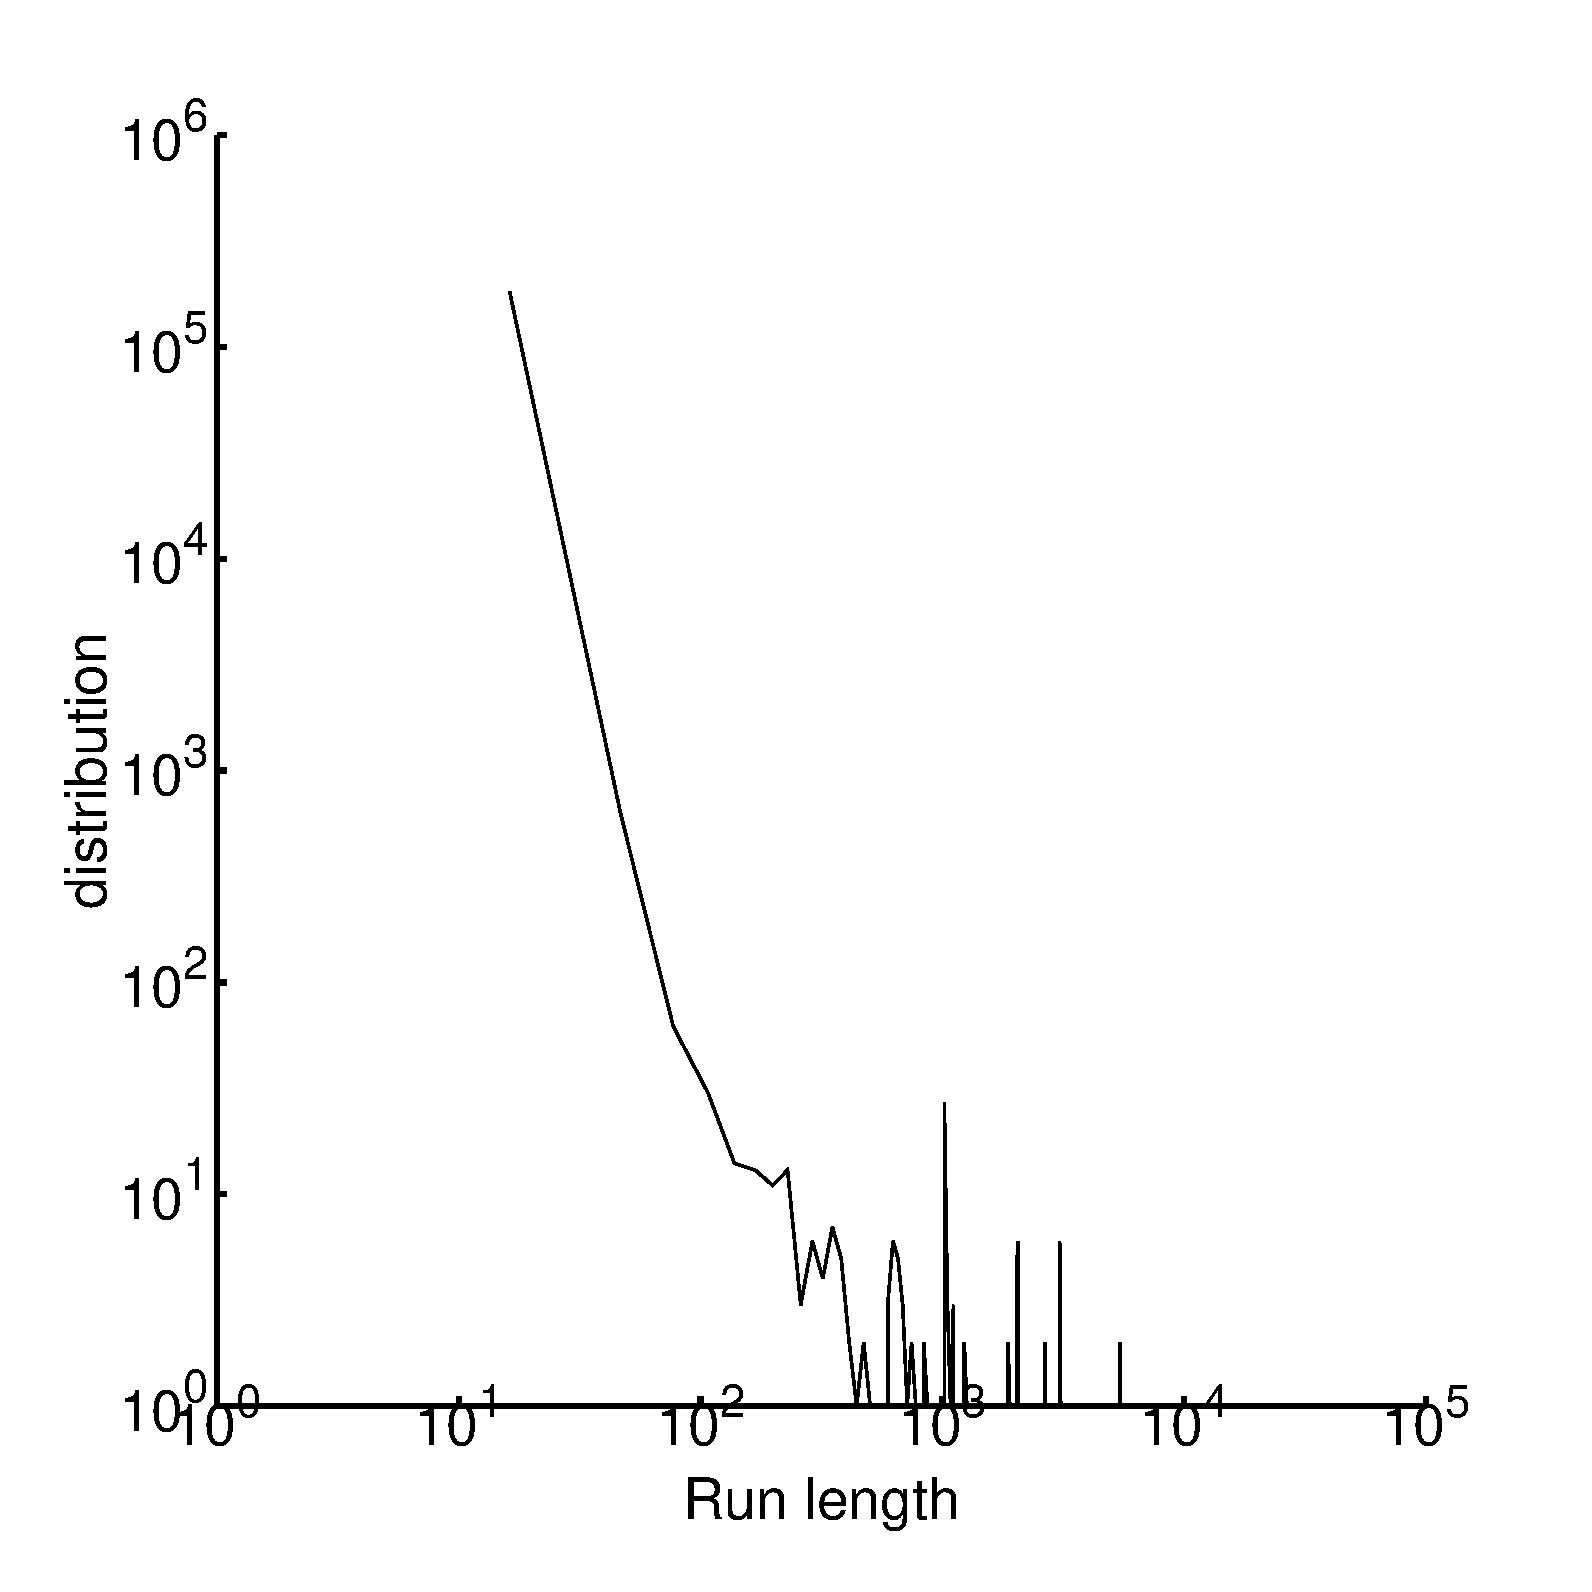
\includegraphics[scale=0.4]{tracechar-figures/3-day/webvm-run-length-distrib-readonly-appended-3-loglog.eps}}
%	\label{fig:webvm-runlength-read-write-distrib}
%\end{figure}

The run length distributions for read and write requests have been 
plotted in Fig.~\ref{fig:webvm-runlength-read-write-distrib}, where it
can be seen that as the run length increases, the number of occurrences
of that run length reduces. More specifically, read request run length
distribution for \textit{webvm} and \textit{homes} reveals
the following important points:-
\begin{enumerate}

	\item Read run length of less than 10 blocks occur close to $10^6$
		times in both \textit{webvm} and \textit{homes} traces
	\item Read run length of between 10 to 100 blocks occur between
		10 to $10^4$ times in both traces
	\item Read run length of greater than 100 blocks occur around 10 times or less
\end{enumerate}
The above observations enable us to conclude that very long run lengths 
in read I/O are rare whereas run length of less than 10 blocks is mostly 
the norm. Our observation of 82\% run lengths being of 1 block also 
corroborates the finding in \cite{storagecharacterization} that most I/O 
in web service applications is found to be random access and not sequential.

The write request run length distribution plotted in 
Fig.~\ref{fig:webvm-runlength-read-write-distrib}(b) 
shows that a similar characteristic (as observed
with reads) is present here as well. The following points may be noted:-
\begin{enumerate}
	\item In both cases, there is a huge number of instances of run length = 1
	\item The maximum write run length is only around 3$\times 10^3$ whereas 
		the maximum read run length is over a magnitude larger at around
		3$\times 10^4$
	\item The maximum run length for reads in \textit{homes} trace is 32,510 blocks compared
      to 1024 blocks for write run length		
\end{enumerate}

To achieve a better comparison across these different plots, we present the
probability distributions below
in Fig.~\ref{fig:runlength-read-write-distrib-prob}, such that the total number of requests 
within the trace doesn't skew the number of instances in each bucket.
In fact, the probability distribution captures which is the most expected
and least expected run length in each of the considered cases.
From Fig.~\ref{fig:runlength-read-write-distrib-prob}, we can see that
\begin{enumerate}
 \item The number of instances of run length = 1 in case of read requests in \textit{webvm}
		trace is proportionally much higher than the corresponding write requests, 
		specifically 86\% in reads as opposed to 57\% in writes
 \item 75\% of the values in the both the read and write run 
      length distribution of \textit{homes} trace are for run length = 1 block
 \item Additionally, the read requests of both the \textit{webvm} and \textit{homes} trace
      have more instances
      of run length less than 10, as compared to the write requests
\end{enumerate}
From the above, we can conclude that, in both the \textit{webvm} and \textit{homes} traces,
read run lengths are generally shorter than write lengths, which is indicated
by the read run length distributions having taller bars for shorter run lengths,
and shorter bars for longer run lengths, in comparison to the write run length
distributions.



%block numbers accessed consecutively, and duplicate content blocks accessed consecutively
\begin{figure}[t]
	\centering
	\subfloat[Block run length for reads (\textit{webvm})]{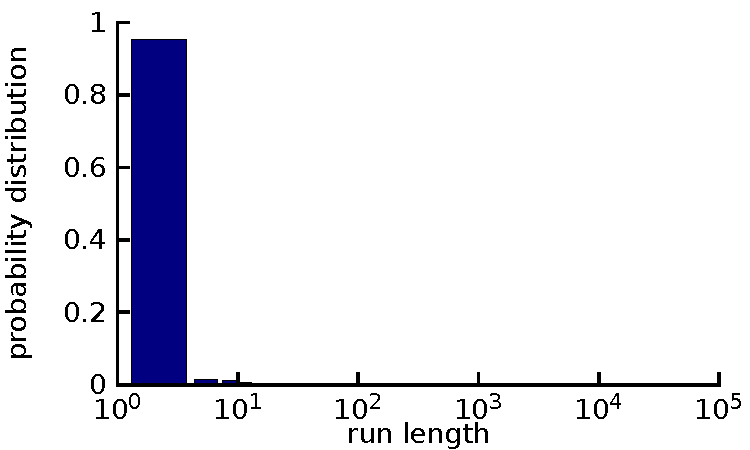
\includegraphics[scale=0.6]{tracechar-figures/21-day/webvm-run-length-distrib-readonly-appended-21-prob.pdf}} 
	\hfill
	\subfloat[Block run length for writes (\textit{webvm})]{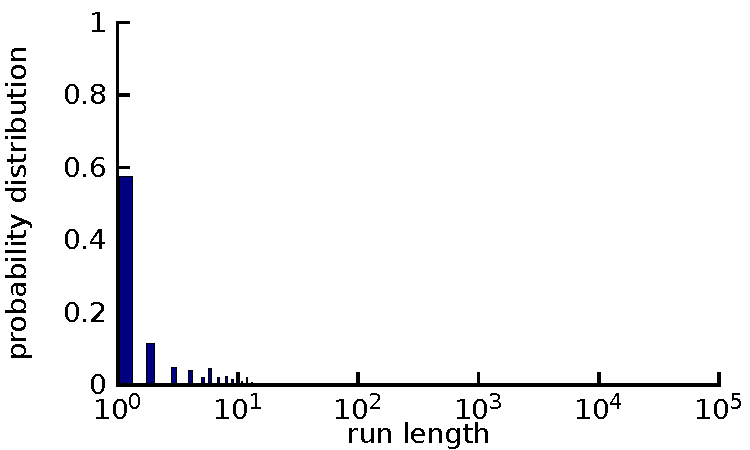
\includegraphics[scale=0.6]{tracechar-figures/21-day/webvm-run-length-distrib-writeonly-appended-21-prob.pdf}}
	\\
	\subfloat[Block run length for reads (\textit{homes})]{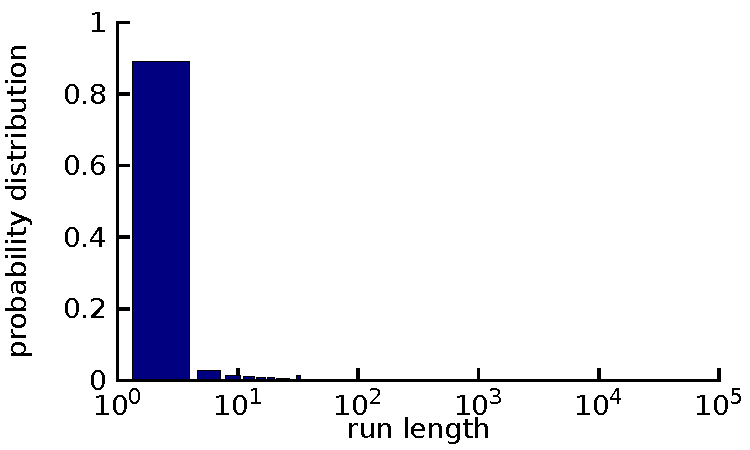
\includegraphics[scale=0.6]{tracechar-figures/21-day/homes-run-length-distrib-readonly-appended-21-prob.pdf}} 
	\hfill
	\subfloat[Block run length for writes (\textit{homes})]{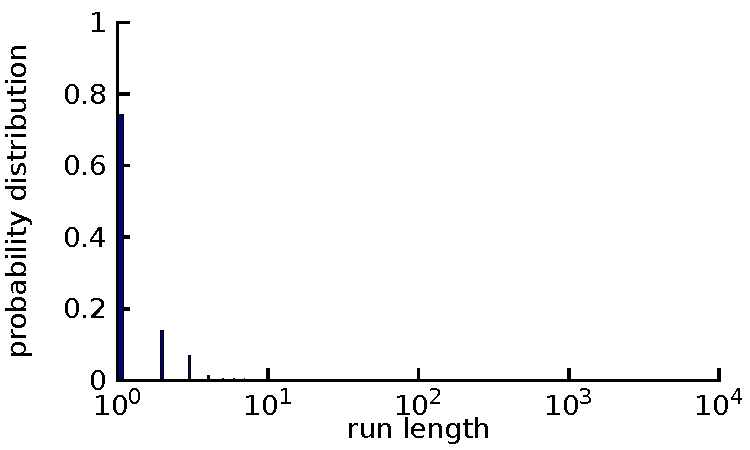
\includegraphics[scale=0.6]{tracechar-figures/21-day/homes-run-length-distrib-writeonly-appended-21-prob.pdf}}
	\caption{\textit{Block run length} probability distribution for reads and writes in \textit{webvm} and \textit{homes} traces}
	\label{fig:runlength-read-write-distrib-prob}
\end{figure}


  
Since our study is geared towards understanding the duplicate content
characteristics of the trace, we further present a content-defined version
of the \textit{run length} metric, which we refer to as the 
\textit{duplicate content run length}. Basically, this metric tries to
capture whether the duplicate content blocks are those that have a run
length of one, or those with longer run lengths.
% , which has further
% implications on whether data access patterns will get fragmented or not 
% due to I/O deduplication. 

By investigating the \textit{duplicate content run length} metric, we
observed that \textbf{all} the 158852 read requests that were found to
have duplicate content in \textit{webvm} trace were of run length = 1 block.
% within the original trace. 
% Thus, we observe that none of the sequences
% with run length greater than 1 got deduplicated.
This is understandable, since most of the read requests in the trace 
were of run length = 1 block as well (86\% as reported above).
% This also shows that there is
% no risk of I/O causing a random access pattern, because the access pattern
% is random even without the I/O deduplication optimization.

%\begin{figure}
%	\centering
%	\includegraphics[scale=0.4]{tracechar-figures/3-day/webvm-dedup-run-length-read-appended-21.eps}
%	\label{fig:webvm-run-length-dedup-distrib}
%	\caption{Distribution of duplicate content run length}
%	\vspace{-0.2in}
%\end{figure}



\subsection{Reuse distance distribution}

\begin{figure}
	\centering
	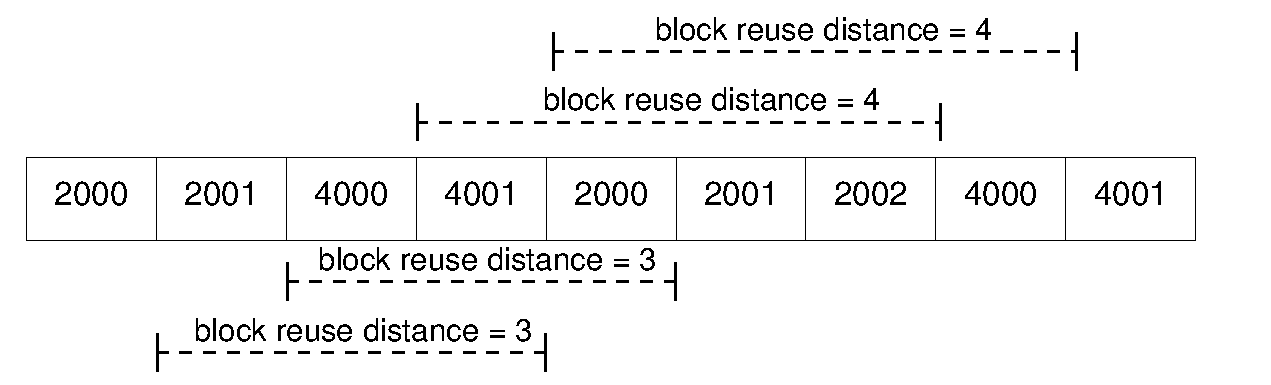
\includegraphics[scale=0.6]{tracechar-figures/21-day/reusedist-example.pdf}
	\caption{Example to explain the definition of \textit{block reuse distance}}
	\label{fig:reusedist-example}
\end{figure}

The term \textit{reuse distance} refers to the number of blocks (or content)
between two successive accesses to the same block (or content)~\cite{iodedup}. 
An example of block reuse distance is
presented in Fig.~\ref{fig:reusedist-example} which shows a series
of blocks\textemdash{}2000, 2001, 4000, 4001, 2000, 2001, 2002, 4000, 4001\textemdash{}being
accessed. In this sequence, the blocks 2000, 2001, 4000 and 4001 have
been ``reused'', i.e., accessed more than once. The reuse distance in
each of these cases is as marked in the figure, i.e. reuse distance
= 3, 3, 4, 4, respectively. Similarly, \textit{content reuse distance}
is defined per access of same content, and is irrespective of its block 
address. Thus, if blocks 2000 and 4000 have duplicate content as shown
in Fig.~\ref{fig:content-reusedist-example}, then content reuse distances
for that content would be 1, 1 and 2 in the given example.

A study of \textit{block reuse distance} versus \textit{content reuse distance}
for the \textit{webvm} trace is present in \cite{iodedup}, however only
``average'' distances are reported whereas we present the ``distribution'' here.
Similar to the observation in \cite{commercial-characterization}, we also
believe that distributions paint a better picture of the overall scenario
than mere averages.


\begin{figure}
	\centering
	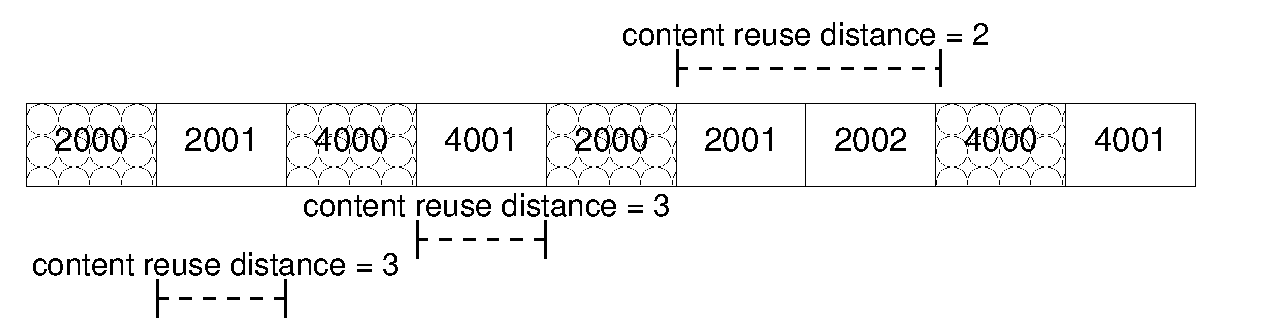
\includegraphics[scale=0.6]{tracechar-figures/21-day/content-reusedist-example.pdf}
	\caption{Example to explain the definition of \textit{content reuse distance}}
	\label{fig:content-reusedist-example}
\end{figure}

\begin{figure}[t]
	\centering
	\subfloat[Read blocks (\textit{webvm})]{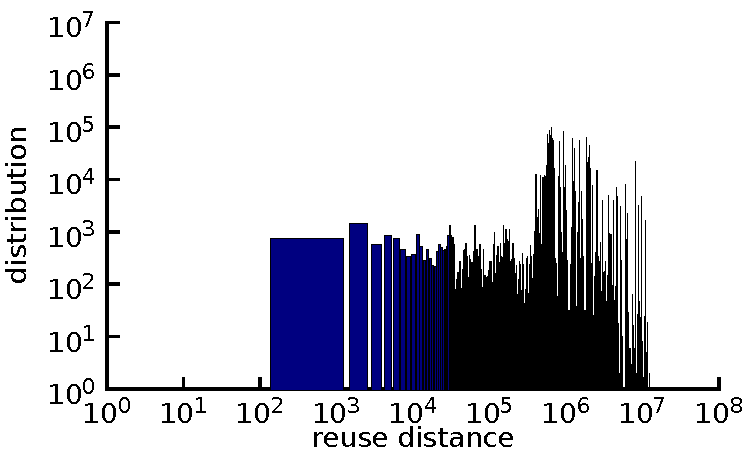
\includegraphics[scale=0.6]{tracechar-figures/21-day/webvm-reuse-dist-distrib-readonly-appended-21-loglog.pdf}} \hfill
	\subfloat[Write blocks (\textit{webvm})]{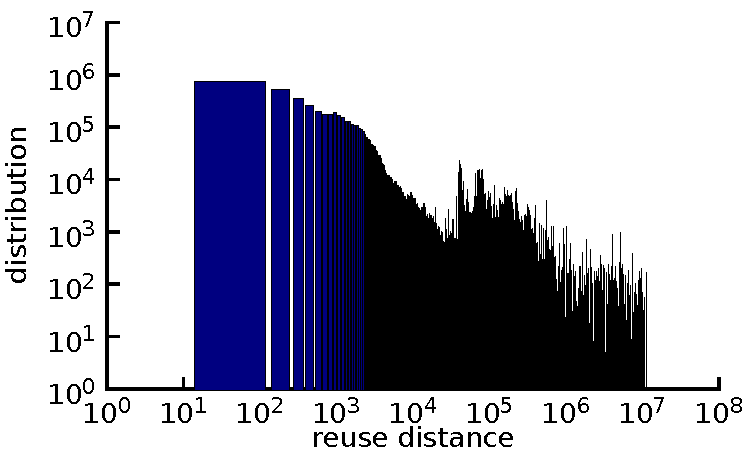
\includegraphics[scale=0.6]{tracechar-figures/21-day/webvm-reuse-dist-distrib-writeonly-appended-21-loglog.pdf}}
	\\
	\subfloat[Read blocks (\textit{homes})]{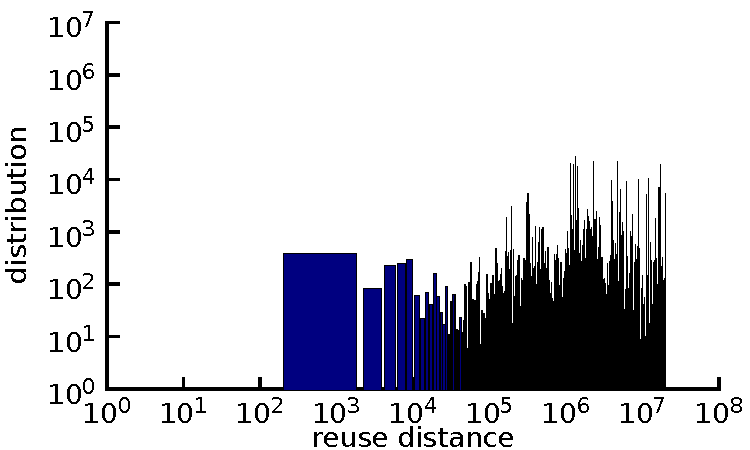
\includegraphics[scale=0.6]{tracechar-figures/21-day/homes-reuse-dist-distrib-readonly-appended-21-loglog.pdf}} \hfill
	\subfloat[Write blocks (\textit{homes})]{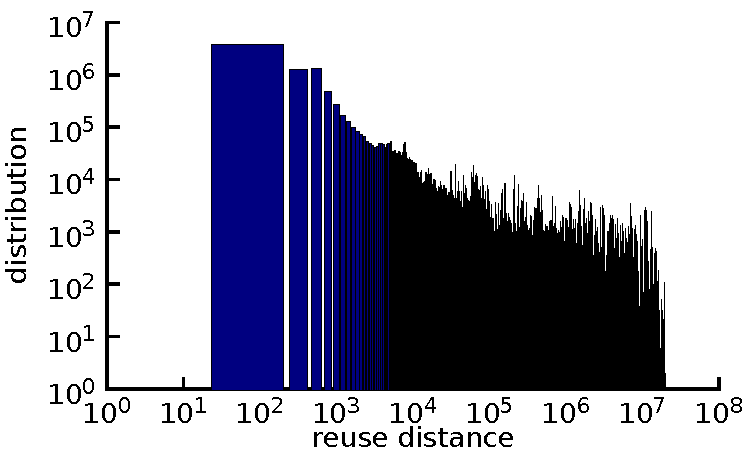
\includegraphics[scale=0.6]{tracechar-figures/21-day/homes-reuse-dist-distrib-writeonly-appended-21-loglog.pdf}}	
	\caption{\textit{Block reuse} distance distribution for reads and writes in \textit{webvm} and \textit{homes} traces}
	\label{fig:reusedist-read-write-distrib}
\end{figure}

The block reuse distance distributions for the read and write requests for
both the \textit{webvm} and the \textit{homes} traces are plotted in
Fig.~\ref{fig:reusedist-read-write-distrib}. 
In both read and write distributions, \textit{webvm} trace has greater occurrence of
smaller reuse distances that the \textit{homes} trace. Also, both traces have 
smaller reuse distances for write requests as compared to read requests. This 
may be because when files are over-written using an editor, its corresponding
blocks that have been fetched into page cache, tend to get freed up and new
blocks allocated for writing the new content~\cite{longterm-fair}. 
The blocks that get freed up thereby, might get re-allocated soon as and when
new write requests come in\textemdash{}this may result in a higher churn of write blocks, 
in write-intensive workloads.


\begin{figure}[t]
	\centering
	\subfloat[Read content (\textit{webvm})]{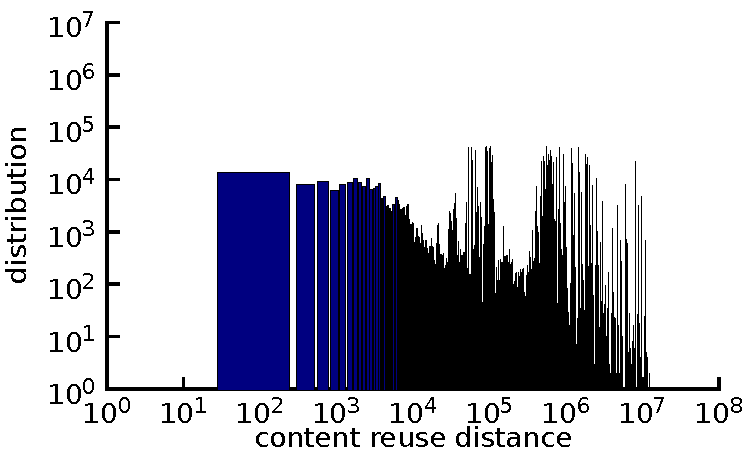
\includegraphics[scale=0.6]{tracechar-figures/21-day/webvm-reuse-dist-distrib-dedup-readonly-appended-21-loglog.pdf}} \hfill
	\subfloat[Write content (\textit{webvm})]{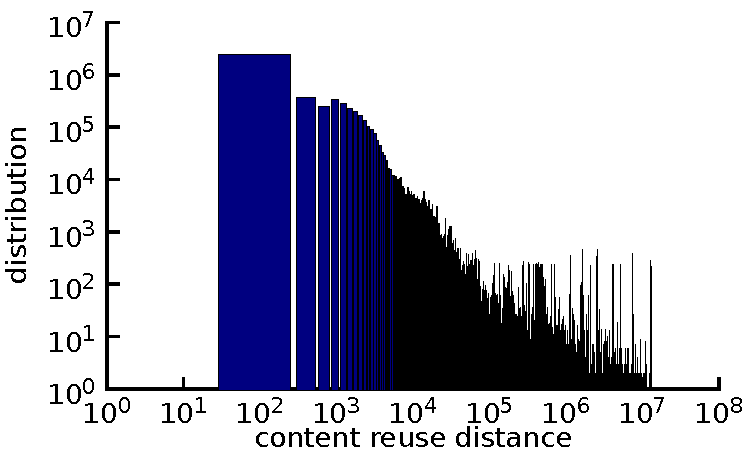
\includegraphics[scale=0.6]{tracechar-figures/21-day/webvm-reuse-dist-distrib-dedup-writeonly-appended-21-loglog.pdf}}
	\\
	\subfloat[Read content (\textit{homes})]{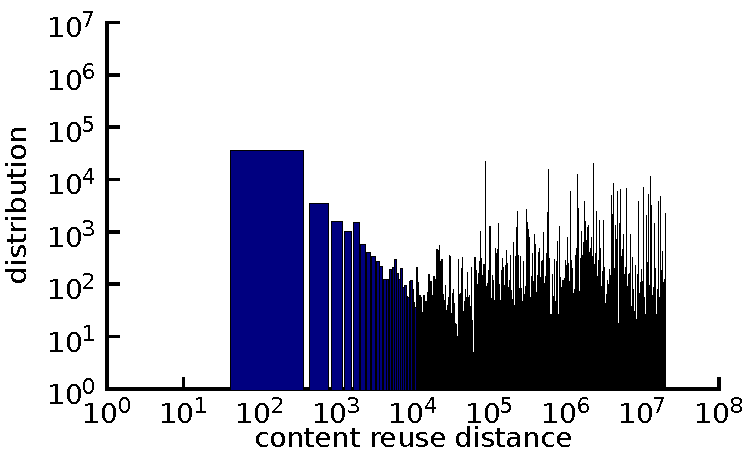
\includegraphics[scale=0.6]{tracechar-figures/21-day/homes-reuse-dist-distrib-dedup-readonly-appended-21-loglog.pdf}} \hfill
	\subfloat[Write content (\textit{homes})]{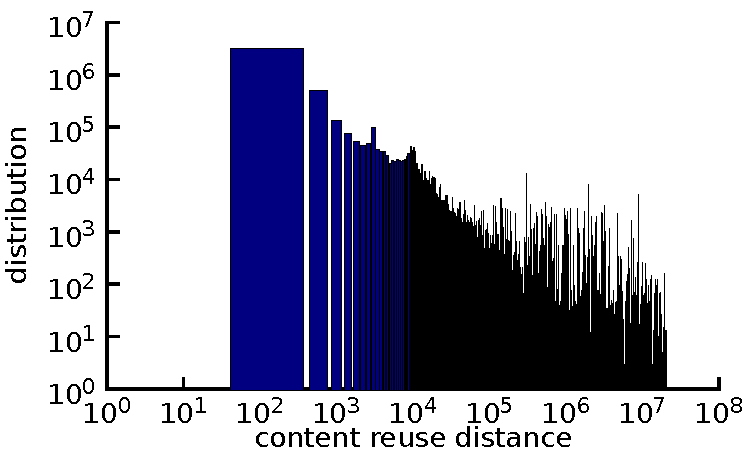
\includegraphics[scale=0.6]{tracechar-figures/21-day/homes-reuse-dist-distrib-dedup-writeonly-appended-21-loglog.pdf}}	
	\caption{\textit{Content reuse} distance distribution for reads and writes in \textit{webvm} trace}
	\label{fig:reusedist-dedup-read-write-distrib}
\end{figure}


As per our observations in Section~\ref{sec:similarity-study} regarding the similarity
study within the three traces, we had concluded that the number of occurrences of
each piece of content was greater than the number of distinct block numbers that
had the same piece of content. In other words, occurrence factor was found to 
be greater than sharing factor for each content. This would imply that the 
distance between accesses to the ``same'' content should be lower than the 
distance between accesses to the same block. To verify this, we present a distribution of 
the content reuse distance in Fig.~\ref{fig:reusedist-dedup-read-write-distrib}.

By comparing each of the graphs Fig.~\ref{fig:reusedist-dedup-read-write-distrib} (a),
(b), (c) and (d) with Fig.~\ref{fig:content-reusedist-example} (a), (b), (c)
and (d), respectively, we can see that in each case, the \textit{content reuse distances}
are smaller than the \textit{block reuse distances}, as expected. Also, the number of
instances of the smallest content reuse distance in each case, is at least an order
of magnitude larger than the number of instances of the smallest block reuse distance,
respectively. Note that, shorter content reuse distance indicates that if the cache
is operated in a content-based manner rather than block-based manner, it would provide
greater benefits~\cite{iodedup}.

\begin{table}[t]
 \caption{Reuse distance statistics for reads in \textit{webvm} and \textit{homes} traces}
%  \hspace{-0.2in}
 \begin{center}
 \begin{tabular}{|c|c|c|c|c|c|} \hline
   \bf{Workload} & \bf{Total} & \bf{Reads with} & \bf{Reads with} & \bf{Reads with} & \bf{Reads with} \\
  \bf{type} & \bf{reads} & \bf{block reuse} & \bf{block reuse} & \bf{content reuse} & \bf{content reuse} \\ 
	    & \bf{(\#)} & \bf{(\#)} & \bf{(\% of total)} & \bf{(\#)} & \bf{(\% of total)} \\ \hline  
  \textit{webvm} & 3,116,456 & 2,800,411 & 90 & 2,873,998 & 92 \\
  \textit{homes} & 4,052,176 & 695,747 & 17 & 732,265  & 18 \\ \hline
 \end{tabular}
 \label{tab:reuse-dist-read-summary}
 \end{center}
 \end{table}
At a high-level view, it may seem that both the \textit{webvm} and \textit{homes}
traces have similar block and content reuse-distance distributions. Note however that,
the axes in these graphs are log-log, so even a ``slight'' difference
can be considered as a significant difference in normal scale. 
To demonstrate that the difference between
them is significant enough to result in differential performance for the two traces, 
we present the statistics in 
Table~\ref{tab:reuse-dist-read-summary} regarding the total number of 
read requests in each trace, and the number of read requests resulting
in block reuse and content reuse in each of them.



\subsection{Jump distance distribution}
In the context of I/O traces, \textit{jump distance} refers to the
distance between successive I/O requests. Specifically, if consecutive
requests are continuous in the logical block address (LBA or LBN) space, 
then the jump distance between them is zero. However, when there are
two consecutive requests (read or write combined) such that they are
not continuous, there is said to be a positive jump distance between
them, equal to the difference between the two block addresses.
Considering the example in Fig.~\ref{fig:jumpdist-example}, we can see
that the given request trace consists of three sequences of 
accesses\textemdash{}2000 to 2002, 2050 to 2054, and 4000. Thus, two non-zero
``jump distances'' can be noted in the example, one after access to
block 2002 and the other after block number 2054.


\begin{figure}
	\centering
	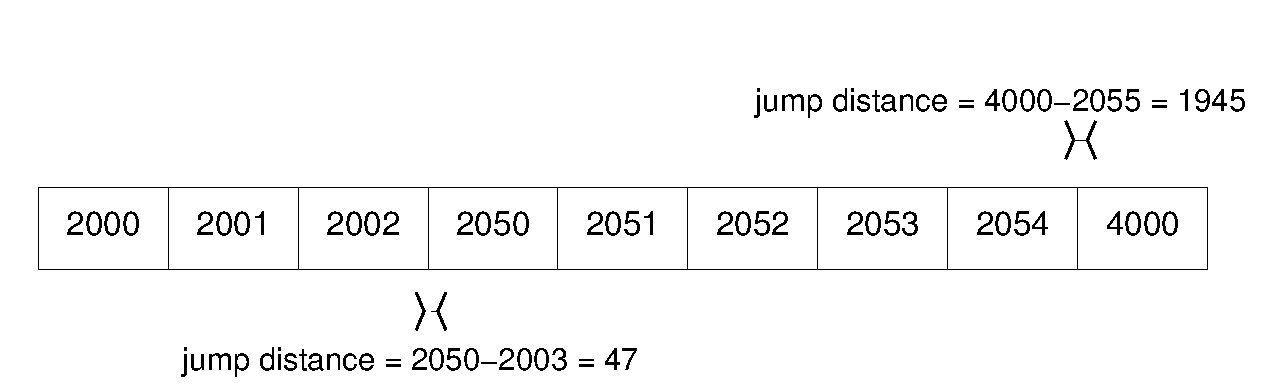
\includegraphics[scale=0.6]{tracechar-figures/21-day/jumpdist-example.pdf}
% 	\vspace{-0.3in}
	\caption{Example to explain the definition of \textit{jump distance}}
	\label{fig:jumpdist-example}
\end{figure}

% \begin{figure}[t]
% 	\centering
% 	\subfloat[Jump distance distribution for block reads]{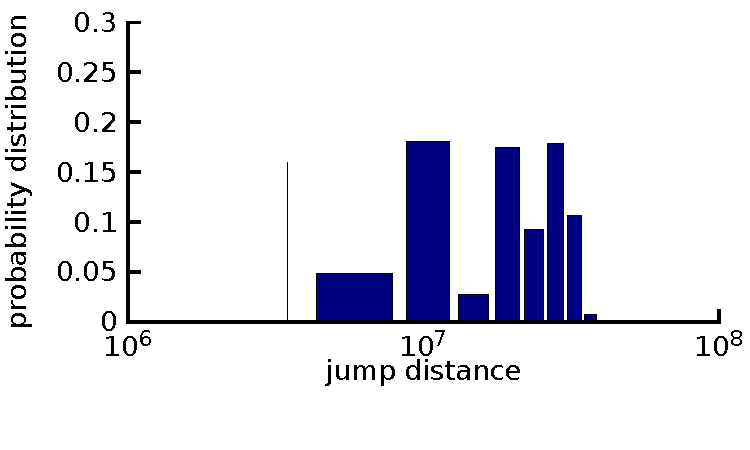
\includegraphics[scale=0.6]{tracechar-figures/3-day/webvm-jump-dist-distrib-readonly-appended-3-prob.pdf}}
% 	\hfill
% 	\subfloat[Jump distance distribution for block writes]{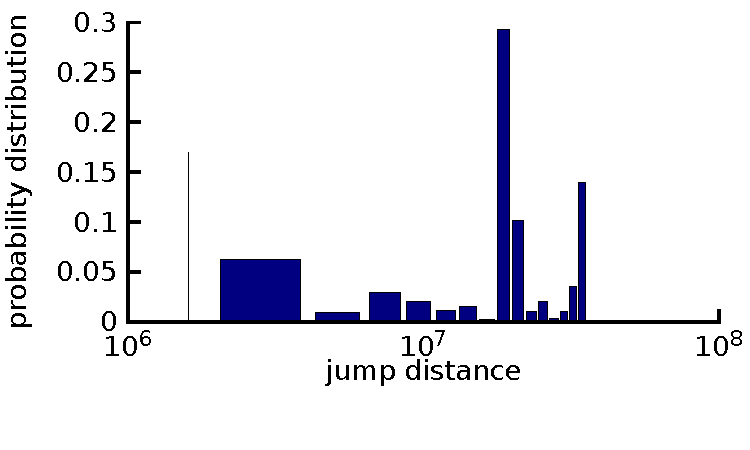
\includegraphics[scale=0.6]{tracechar-figures/3-day/webvm-jump-dist-distrib-writeonly-appended-3-prob.pdf}}
% 	\label{fig:webvm-jumpdist-read-write-distrib}
% \end{figure}

\begin{figure}
	\centering
	\subfloat[Jump distance distribution for \textit{webvm} trace]{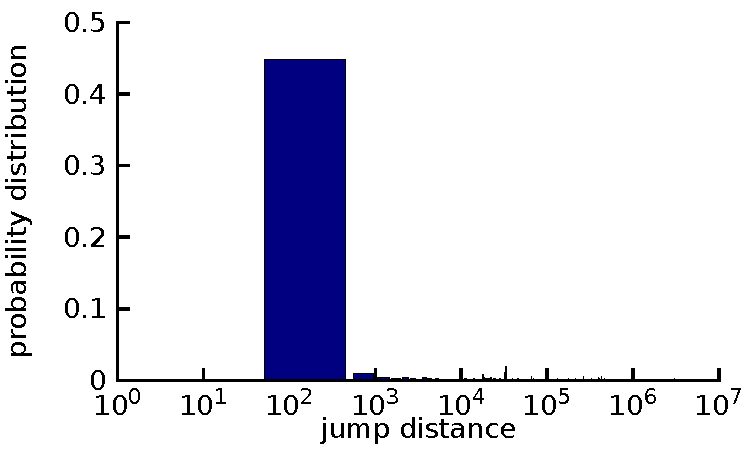
\includegraphics[scale=0.6]{tracechar-figures/21-day/webvm-jump-dist-distrib-readwrite-appended-21-prob.pdf}}
	\hfill
	\subfloat[Jump distance distribution for \textit{homes} trace]{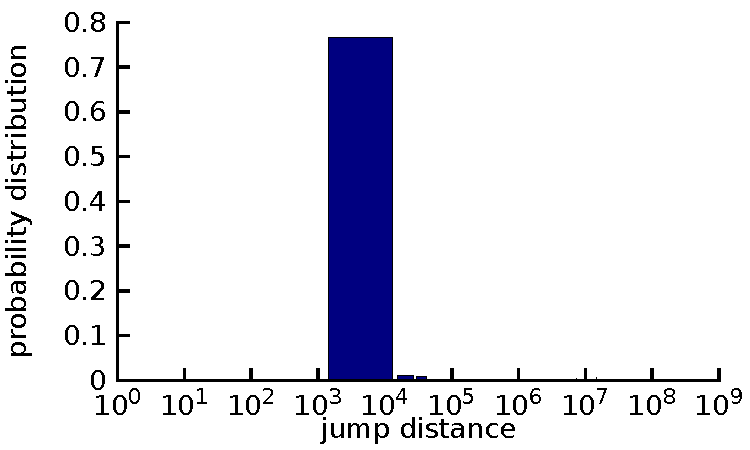
\includegraphics[scale=0.6]{tracechar-figures/21-day/homes-jump-dist-distrib-readwrite-appended-21-prob.pdf}}
	\caption{Jump distance probability distribution for read/write trace of \textit{webvm} and \textit{homes}}
	\label{fig:jumpdist-read-write-distrib}
\end{figure}

Although for all of the above metrics, we had presented separate distribution
for reads and writes, here we present a single distribution for all reads
and write requests combined. This is similar to the approach adopted 
in \cite{case-for-nas-benchmarks} and makes sense because jump distance
is a characteristic of the access trace which indicates how randomly or
not, the blocks are accessed (read or written) in the workload.

Fig.~\ref{fig:jumpdist-read-write-distrib} presents the probabilistic jump
distance distributions for both the \textit{webvm} and the \textit{homes} traces.
We can see that the majority of jump distances in the \textit{webvm} trace lie
between 100 to 1000 whereas they are between 1000 to 10,000 for the \textit{homes}.
Moreover, the largest jump distance in the \textit{homes} trace is an order of magnitude
larger than the largest jump distance in the \textit{webvm} trace. This is possibly
because the filesystem of the \textit{homes} system is similarly 
larger (470 GB) than the \textit{webvm} system (70 GB),
as mentioned earlier in Table~\ref{tab:tracechar-summary-stats}.

In this section, we described various characteristics of the I/O traces and 
quantified their content-defined versions for the available \textit{homes} and
\textit{webvm} traces. In the next section, we make the case that we need to
use such characterization to generate synthetic traces for evaluating new
I/O deduplication techniques comprehensively.
